\documentclass[fontsize=12pt,paper=letter,cleardoublepage=plain,twoside=false]{scrbook}

% adapted from https://github.com/jonhoo/thesis/

% for 1.5 line spacing
\usepackage{setspace}
\onehalfspacing
% single spacing for table of contents
\AfterTOCHead{\singlespacing}

% recompute page layout based on the above
\recalctypearea

% more colors (like RedOrange)
\usepackage[dvipsnames]{xcolor}

% qualitative colors
% subset of https://jfly.uni-koeln.de/color/
% that is also distinctive in grayscale
\definecolor{set1}{HTML}{0071b2} % blue
\definecolor{set2}{HTML}{e59c00} % orange
\definecolor{set3}{HTML}{009e73} % green
\definecolor{set4}{HTML}{efe440} % yellow

% so we can splice in PDFs
\usepackage{pdfpages}

% set up bibliography
\usepackage[square,comma,numbers,sort&compress]{natbib}

% enumerate* and itemize*
\usepackage[inline]{enumitem}

% for \begin{comment}
\usepackage{verbatim}

% for source-code listings
\usepackage[newfloat,draft=false]{minted}

% for formulas
\usepackage{mathtools}

% to split lists into multiple columns
\usepackage{multicol}

% for "on page NN" reference
\usepackage[nospace]{varioref}

% for \sfrac
\usepackage{xfrac}

% for \ifoptionfinal
\usepackage{ifdraft}

\usepackage[breaklinks, pdfborder={0 0 0}]{hyperref}
\usepackage[nameinlink]{cleveref}

% for \num, used in \loc macro
\usepackage[group-separator={,}]{siunitx}

% generate synctex output for inverse search
\synctex=1

% an environment for todos
\newenvironment{inprogress}
  {\vspace{.5em} \color{set2} \noindent \textbf{TODO}}
  {\vspace{.5em}}
\newcommand{\insertnote}[3]{\noindent\textcolor{#1}{\textbf{#2:} #3}}
\newcommand{\note}[1]{\insertnote{blue}{NOTE}{#1}}
\newcommand{\todo}[1]{\insertnote{red}{TODO}{#1}}

% a command to indicate current editing progress
\newcommand{\resume}{
  \begin{center}
    \color{set2}
    \hrule
    \vspace{1pt}
    \hrule
    \hrule
    \vspace{10pt}
    \textbf{This section is not yet complete.}
    \vspace{10pt}
    \hrule
    \hrule
    \vspace{1pt}
    \hrule
  \end{center}
}

\usepackage{relsize}
\renewcommand{\ttdefault}{pxtt}
\newcommand{\horizontalrule}{\rule{\textwidth}{0.5pt}}

%% semantic formatting
\newcommand{\code}[1]{\texttt{\detokenize{#1}}}
\newcommand{\cc}[1]{\mbox{\smaller[0.5]\texttt{\detokenize{#1}}}}
\newcommand{\scc}[1]{\mbox{\textsc{\detokenize{#1}}}}
\npthousandsep{,}
\newcommand{\loc}[1]{\numprint{#1}}

% \newidentmacro{foobar} creates \foobar that expands to foobar, with the right
% formatting to be an identifier.
\newcommand{\newidentmacro}[1]{\csdef{#1}{\mathtt{#1}}}
% \newdefmacro{foobar} is like \newidentmacro but it uses textlog to format the
% identifier
\newcommand{\newdefmacro}[1]{\csdef{#1}{\textlog{#1}}}

\newcommand{\tightenspace}{\vspace{-\baselineskip}}

%% Code

\newcommand{\load}[1]{\operatorname{Load}(#1)}
\newcommand{\store}[2]{\operatorname{Store}(#1, #2)}

%% notation

% https://tex.stackexchange.com/questions/4194/how-to-typeset-haskell-operator-and-friends
\newcommand\mdoubleplus{\ensuremath{\mathbin{+\mkern-10mu+}}}
\newcommand{\mapupd}[2]{[#1 \mapsto #2]}

%% iris.sty extensions for Perennial

\newcommand{\sep}{*}

% \newcommand{\wpc}[3]{\operatorname{wpc} \, #1 \, \{#2\} \, \{#3\}}
\NewDocumentCommand\wpc{O{} m O{} o m m}%
  {\textlog{\syntax{wpc}}^{#1}_{#3\IfValueT{#4}{,#4}}\spac#2\spac{\syntaxbraced{#5}}\spac{\syntaxbraced{#6}}}

\newcommand{\recoverwith}{\circlearrowleft}
\NewDocumentCommand\wpr{O{} m m O{} m m}%
  {\textlog{\syntax{wpr}}^{#1}_{#4}\spac#2 \recoverwith #3 \spac{\syntaxbraced{#5}}\spac{\syntaxbraced{#6}}}

\newcommand{\wpcw}{\textlog{wpc}\xspace}
\newcommand{\wprw}{\textlog{wpr}\xspace}
\newcommand{\wpw}{\textlog{wp}\xspace}

\newcommand{\notval}[1]{\neg \textlog{value(#1)}}
\newcommand{\cbmask}{\textlog{B}}

\NewDocumentCommand \hoareC {m m m m}{
  \curlybracket{#1}\spac #2 \spac \curlybracket{#3}\curlybracket{#4}%
}

\NewDocumentCommand \hoareCV {O{c} m m m m}{
  {\begin{aligned}[#1]
      &\curlybracket{#2} \\
      &\quad{#3} \\
      &\curlybracket{#4} \\
      &\curlybracket{#5}
    \end{aligned}}%
}

\newcommand{\postcrash}{\mathop{\blacklozenge}}
\newcommand*{\preborrow}{\textlog{preborrow}}
%\newcommand*{\cInv}[2]{{\boxedassert{#1 \mathop{|} #2}}^{\lightning}}
\newcommand*{\cInv}[2]{{\boxedassert{#1 \mathop{|} #2}}}
%\NewDocumentCommand \cfupd {O{} O{}} {\mathord{{}^\lightning\kern-1.15ex\vsGen[]{{\mid\kern-0.5ex\Rrightarrow\kern-0.25ex}}^{#1}_{#2}\kern0.2ex}}

\newcommand{\SKIP}{\mathit{noop}}
\renewcommand{\Ret}[1]{\text{\textbf{ret}}\,\, #1,\,}

%% more Perennial stuff

\newcommand{\lock}[1]{\textlog{acquire}(#1)}
\newcommand{\unlock}[1]{\textlog{release}(#1)}
\newcommand{\newlock}{\textlog{newlock}()}

\newcommand{\prelock}[1]{\textlog{preLock}(#1)}
\newcommand{\islock}[2]{\textlog{isLock}(#1, #2)}
\newcommand{\locked}[1]{\textlog{locked}(#1)}

%\newcommand{\precrashlock}[1]{\textlog{preCrashLock}(#1)}
\newcommand{\iscrashlockNoArgs}{\textlog{isCrashLock}}
\newcommand{\iscrashlock}[3]{\iscrashlockNoArgs(#1, #2, #3)}
\newcommand{\crashlockedNoArgs}{\textlog{crashLocked}}
\newcommand{\crashlocked}[3]{\crashlockedNoArgs(#1, #2, #3)}
\newcommand{\precrashlock}[1]{\textlog{preCrashLock}(#1)}

% Disk FFI
\newcommand{\diskwriteNoArgs}{\textlog{DiskWrite}}
\newcommand{\diskreadNoArgs}{\textlog{DiskRead}}
\newcommand{\diskwrite}[2]{\diskwriteNoArgs(#1, #2)}
\newcommand{\diskread}[1]{\diskreadNoArgs(#1)}
\newcommand{\dmapsto}{\mapsto_\textsf{d}}
\newcommand{\vals}{vs}
\newcommand{\block}{b}
\newcommand{\addr}{a}

\newcommand{\memory}{m}
\newcommand{\disk}{d}

% newly defined here (durable(P) := P |- post_crash(P))
\newcommand{\durable}{\textlog{durable}}

%%% GoJournal

% abbreviations
\newcommand{\fstar}{F${}^\star$\xspace}
\newcommand{\lowstar}{Low${}^\star$\xspace}
\newcommand{\lambdarust}{$\lambda_{\mathrm{Rust}}$\xspace}
\newcommand{\safe}{\mathrm{safe}}

% GoJournal total
\newcommand{\gotxnLOC}{\loc{1345}}
\newcommand{\gotxnLOP}{\loc{25797}}
%

%%% DaisyNFS

% soundness definitions
\newcommand{\refines}{\sqsubseteq}
\newcommand{\progeq}{\approx}

% ``type arg'', to write something like Goose<L>. I'm using angle brackets to
% match C++ and Rust.
\newcommand{\targ}[1]{\langle #1 \rangle}
\newcommand{\layer}{L}
% the type of operations O
\newcommand{\OP}{\mathcal{O}}
\newcommand{\crash}{\operatorname{crash}}
\newcommand{\gooselayervar}[1]{\ensuremath{\mathtt{Go}\targ{\mathit{#1}}}}
\newcommand{\gooselayer}[1]{\ensuremath{\mathtt{Go}\targ{\mathrm{#1}}}}
\newcommand{\compile}{C}
\newcommand{\impl}{I}
\newcommand{\init}{\operatorname{init}}

\newcommand{\server}{\texttt{s}}
\newcommand{\sdfy}{\ensuremath{\server_{\mathrm{dfy}}}}
\newcommand{\sdfyAlt}{\ensuremath{\tilde{\server}_{\mathrm{dfy}}}}
\newcommand{\stxn}{\sdfy}
\newcommand{\ssys}{\ensuremath{\server_{\mathrm{sys}}}}
\newcommand{\snfs}{\ensuremath{\server_{\mathrm{NFS}}}}
\newcommand{\infs}{\ensuremath{i_{\mathrm{NFS}}}}
\newcommand{\txncode}{\texttt{txn}}
\newcommand{\linked}[1]{\ensuremath{\mathrm{link}(#1, \txncode)}}
\newcommand{\linkedcode}{\linked{\sdfy}}
\newcommand{\Sys}{\mathit{Sys}}
% op as a variable
\newcommand{\opv}{\mathit{op}}

\newcommand{\seqrefinement}{\operatorname{seq\_refinement}}
\newcommand{\seqrefinementdfy}{\seqrefinement_{\mathrm{dfy}}}

\newcommand{\atomically}[1]{\ensuremath{\mathtt{atomically}\,\{\, #1 \,\}}}
\newcommand{\atomiccomp}{\mathtt{atomically}\circ}

%%% Goose

% spacing for application
\newcommand{\app}{\:}
\newcommand{\seq}{;\,}
\newcommand{\defeq}{\triangleq}
\newcommand{\lappend}{\mdoubleplus}

\newcommand{\goosedef}[1]{\mathsf{#1}}
\newcommand{\goosekw}[1]{\ensuremath{\goosedef{\textcolor{blue}{#1}}}}
\newcommand{\goosetrue}{\goosekw{true}}
\newcommand{\goosefalse}{\goosekw{false}}

% \gooseif{c}{e1}{e2} -> if c then e1 else e2
\newcommand{\gooseif}[3]{\goosekw{if} \app #1 \app%
  \goosekw{then} \app #2 \app \goosekw{else} \app #3}

% \gooselet{x}{e1}{e2} -> let x = e1 in e2
% the random extra {}'s around the = are so that LaTeX doesn't group anything
% with it (eg, let tmp = !x)
\newcommand{\gooselet}[3]{\goosekw{let} \app #1 {} = {} #2 \app \goosekw{in} \app #3}


% for handy reference
%
% paragraph without spacing:
% \setparsizes{0pt}{0pt}{0pt plus 1fil}

% in thesis: titlehead, subject, title, subtitle
\title{Verifying a concurrent, crash-safe file system with sequential proofs}
\author{Tej Chajed}
\begin{document}

\mainmatter

File systems are an important service of the operating system, yet
implementations still have bugs that lead to incorrect results or even data loss. Formal
verification offers a promising solution by showing that the file system always
meets its specification, even though the implementation has concurrency and
should tolerate a crash or power failure at any time. This thesis introduces
techniques for making such a proof feasible and efficient, with a new
verification framework and novel file-system design that isolates the most
difficult reasoning to a transaction system that provides atomic updates and
then connects to sequential proofs for the correctness of the main file-system
logic.

% Suggested outline for proposal:
%
% - a few paragraphs providing an intro to the chapter
% - motivation
% - approach
% - state of the art
% - challenges
% - overview of design
% - contributions
% - overview of rest of thesis


\chapter{Thesis proposal}
One crucial service in an operating system is its \emph{file system}, the
software that implements the abstraction of files and directories on top of a
disk, which simply stores a long sequence of bytes. File systems are important
because they are used by all applications to store data, and bugs in file
systems are especially costly because they can lead to data loss for any of
these applications. One approach to improve reliability is to use formal
verification, in which the file system is developed along with a proof that it
always follows a high-level specification of its intended behavior. This thesis
develops new techniques to address the key challenges in a file system of
reasoning about \emph{concurrency} and unexpected \emph{crashes} where the whole
computer reboots, a verified transaction system that handles these concerns, and
a file system that uses the transaction system. The final artifact is DaisyNFS,
a verified file system that comes with a proof of correctness and that achieves
good performance.

\section{Motivation}
\label{sec:intro:motivation}

A file system is an especially critical system for
three reasons. First, the file system is widely used --- essentially all applications have
data that is ultimately stored in a file system. Second, implementations are
concurrent and optimized, which increases the potential for bugs. Finally, bugs
are particularly costly since they can lead to permanent data loss for any
application running on top.

Two challenges make implementing a correct file system challenging: crashes and
concurrency. A file system is generally expected to keep application data safe
even if the system stops running at any time, say due to a power failure or
kernel panic. This thesis uses ``crash'' to refer to any of these circumstances
where the computer stops and is rebooted. After a reboot, the file system is
expected to preserve data from before the crash. The second big challenge is
concurrency in the implementation, which complicates approaches for improving
reliability, including both testing and verification.

Bugs are still discovered in widely used file systems like ext4 and btrfs,
despite a long history of developing, testing, and using these file systems. A
recent approach for fuzzing file systems~\cite{kim:hydra} found new crash-safety
issues in both ext4 and btrfs, despite not testing for concurrency issues. A
study conducted in 2013 looked at all patches for Linux file systems from
2005--2013~\cite{lu:fsstudy}, finding hundreds of these patches were to fix bugs
(for example, 450 for ext4 and 358 for btrfs). About 60\% of these bugs lead to
data loss or crash the kernel (and as the study points out, these are much more
serious consequences than most bugs in application software). File systems have
a lot of internal concurrency for performance reasons, which both leads to bugs
and makes testing and fuzzing more challenging.

The approach in this thesis to make a reliable file system is to use formal
verification. In this approach, we write the code, then a specification of the
intended behavior of the code, and finally a mathematical proof that shows the
code always meets the specification. For confidence in the proof itself, the
proof is carried out in a computer and a piece of software called a proof
assistant checks that the proof is valid. The nature of formal verification
forces the proof engineer to systematically cover every corner case in the code.
As a result, they can completely rule out whole classes of bugs, including
low-level bugs like memory safety but also logic errors like returning the wrong
data. Verification does not guarantee that a system is bug-free, because the
specification must be correct and the assumptions in the proof must hold in
practice, but it does help since the specification is smaller than the
implementation, and it isolates debugging to identifying where the specification
is wrong or an assumption was violated.

While the idea of formal verification is not new, there was essentially no
support for reasoning about the combination of crashes and concurrency when this
thesis work started (in 2015). Thus this thesis develops new techniques to
reason about the combination in the first place. We apply these techniques to
DaisyNFS, a verified implementation of the Network File System (NFS) protocol, a
standard file-system interface.

The key to verifying a system with the complexity of DaisyNFS is a design
that splits the file system into two main parts: a transaction system called
GoTxn that makes it easy to get atomicity over the disk, and then the rest of
the file system implemented using a transaction per operation. GoTxn must face
the key challenges of crash safety and concurrency, but it handles them in such
a way that the code on top is verified using comparatively much simpler
sequential reasoning. The file-system code then focuses on implementing features
like the details of the NFS semantics, large files, and efficient data
structures.

\section{State of the art}
\label{sec:intro:related}

Production file systems are generally validated by testing. While testing is
indispensable for development, the nature of a file system makes it difficult to
catch all bugs with only testing. The fundamental difficulty is a high degree of
non-determinism from two sources: crashes in the middle of execution, and
concurrency in the implementation that is needed for good performance.

The importance of file-system correctness has been recognized by the academic
community, thus there are many approaches for increasing confidence with
improved testing. One line of work has explored systematically testing crashes
at intermediate points~\cite{mohan:crashmonkey,pillai:appcrash,yang:explode}. Another line of
work has focused on fuzz testing as a way to induce crash-safety
bugs~\cite{xu:janus,kim:hydra}. These approaches have been successful for
finding bugs, including crash-safety bugs, but they only test sequential
executions, missing bugs due to concurrently issued operations or from crashes
that interrupt multiple operations. Furthermore, unlike formal verification, testing cannot
cover all executions of a program, even without crashes and concurrency,
potentially missing bugs.

The research community has also recognized the value of formal verification for
reasoning about a file-system implementation. The closest related work is
Flashix~\cite{bodenmuller:concurrent-flashix}, a verified, concurrent file
system that runs on flash devices. The techniques
developed to verify Flashix are specialized to its particular file-system
design, especially its write-back cache. Its concurrency is primarily between
regular operations and garbage collection, and read-only concurrency. This
thesis develops a general logic for reasoning about crashes and concurrency and
applies this logic to verify a system with write-write concurrency.

There are other verified file systems, especially the sequential file systems
FSCQ~\cite{chen:fscq} and Yggdrasil~\cite{sigurbjarnarson:yggdrasil} and an
concurrent but in-memory file system AtomFS~\cite{zou:atomfs}. These systems use
verification techniques that do not support both crashes and concurrency, and they
cannot be extended them in a straightforward way to support the other form of reasoning.

\section{Approach}
\label{sec:intro:approach}

What does it mean to give a machine checked, formal proof of a system? At a high
level, program proofs always have three components: an implementation, a
specification, and a proof. When doing machine-checked proofs, all three are
physically represented as code in a verification system. The verification system
checks the proof against the implementation and specification, ensuring that the
proof is complete.

This thesis integrates interactive, foundational proofs using custom
infrastructure (in Coq) as well as automated verification using a
verification-aware programming language (Dafny). These are both machine-checked,
formal proofs, but the interaction models of the two systems are different
enough that this section describes them separately.

In Coq, the core feature is proofs based on dependent type theory, which is
expressive enough to represent essentially any math. A first step when using Coq
is to connect the code to the reasoning in the proof assistant. The particular
approach in this thesis translates executable code to a model in Coq,
implemented by a tool called Goose. The model
and its semantics encodes the
assumptions the proof makes about how the program behaves. The semantics is typically structured as a transition
system, where an execution is a sequence of states the program goes through
along with some notion of observable behavior, like external I/O or return
values. \tej{maybe add a figure of an execution trace}

Once we have a program in Coq, we can reason about it. The goal of
verification is to prove that the program meets its specification, and
where the specification describes the allowed behaviors of the program. The
specifications in this work forbid universally incorrect behavior, like reading an
out-of-bounds address in an array, but more precisely specify what the program
is supposed to do, for example how it responds to user requests.

A common structure to tame the complexity of reasoning about a program is to use
a \emph{program logic}. In principle it might be possible to prove a theorem
about all the behaviors of a program directly, but such a proof would too
complex to be feasible. The program logic organizes the proof with a structured
way of expressing and proving statements about the program, such as breaking the
proof down into theorems about individual functions. The proof in a program
logic will often mirror the structure of the code, since each function has its
own specification and groups of related functions have related specs.

Program logics for concurrency are still an active area of research; only
recently have they reached the maturity to give completely mechanized proofs of
moderate-sized programs. There are few logics that also can reason about crash
safety. Our approach in this thesis is to build a new program logic called Perennial with all the
concurrency-reasoning features of a modern program logic, plus new features for
reasoning about crashes. What makes this feasible is Iris, a modular framework
for concurrency. Iris includes a concurrent program logic which we are able to
extend with crash-safety reasoning while preserving the concurrency reasoning
features, without reimplementing them from scratch.

Using our new program logic, we verified GoTxn, a concurrent transaction system.
The transaction system's correctness theorem says that any program that uses
transactions really has transactional behavior: its execution is equivalent to a
version of the program where the transactions run atomically. The complete
specification includes some important details in order to formalize the
intuition behind atomicity.

Next, because transactions appear to run sequentially, and write to disk all at
once, it is no longer necessary to use a sophisticated program logic like
Perennial to reason about the body of each transaction. Instead, we switch to
using Dafny, a verification-oriented programming language that only supports
sequential code but as a result is highly productive for this use case. The file
system is written and verified in Dafny, then compiled to Go and linked with
GoTxn.

Dafny verification works quite differently from Coq. Dafny is a programming
language with verification features; contrast this with Coq, which supports
general math that can \emph{model} programs. A Dafny method can be annotated
with a specification. The Dafny checker converts a method and its specification
to a logical formula (called a verification condition), which is true if and only if the specification holds for
the method. It then queries a \emph{solver} (Z3, in the case of Dafny) to determine if the formula is true.
Contrast all of this with Coq, where the user manually develops the program
logic and connects the rules of this logic. Checking a program against its specification in Dafny cannot be perfectly
automated because it is impossible to answer whether a general logical formula
is true or not, but the user can insert annotations to help out the solver, and
generally fewer annotations are needed than lines of proof for Coq. The main
downside to this approach is that it fixes a sequential programming language, so
unlike in Coq, it isn't possible to reason about concurrency and crashes.

\Cref{fig:overview} depicts how all of the components of DaisyNFS and its proof
fit together. The left-hand side depicts the implementation, split between GoTxn
and the file-system implemented in Dafny. The Dafny code is compiled to Go and
then the two parts are linked together into one \cc{daisy-nfsd} binary in the
usual Go build process. GoTxn is translated to a model using a tool called
Goose. The right-hand side of the figure depicts all aspects related to the
proof, which is written using the Perennial program logic. All of this happens
in the Coq proof assistant, which checks that the proofs are valid. Meanwhile
the DaisyNFS file-system code is verified in Dafny, which integrates
implementing, specifying, and verifying code. This proof is checked by the Dafny
verifier. Finally, the proof of GoTxn is written in such a way that it can be
composed with the proof of DaisyNFS for a theorem about the whole
\cc{daisy-nfsd} binary. This is a conceptual composition, not one in either
Dafny or Coq.

\begin{figure}[ht]
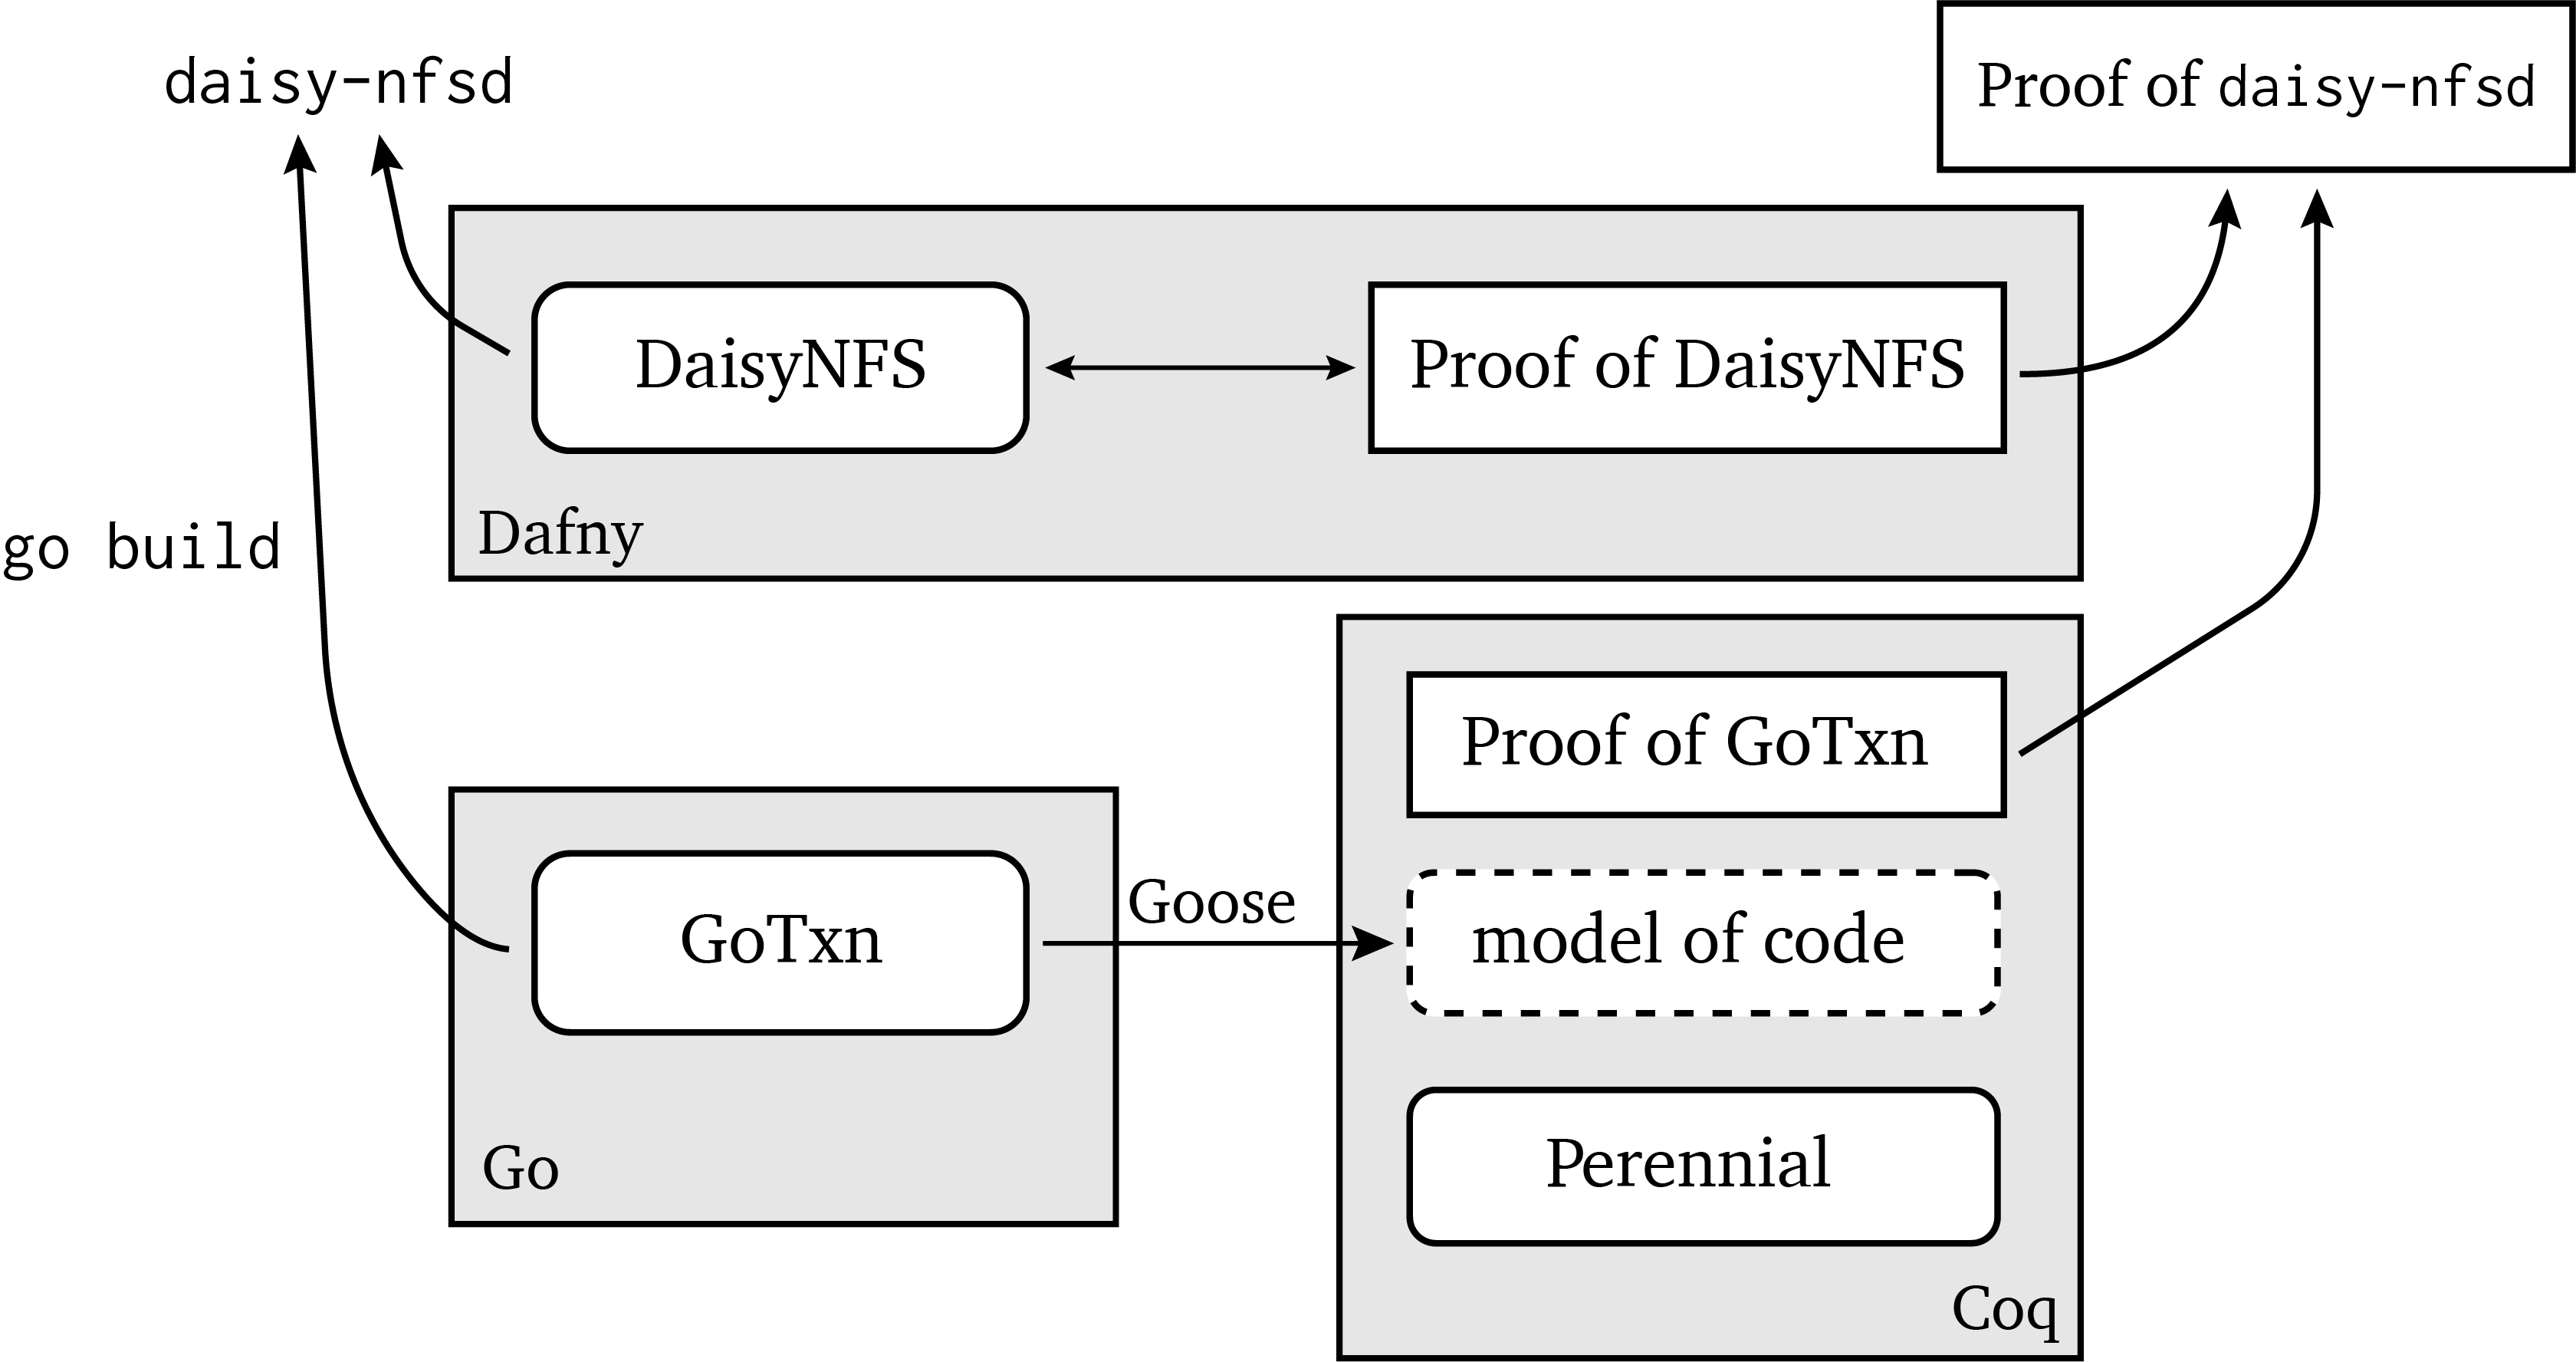
\includegraphics{fig/overview.png}
\caption{Overview of how GoTxn, DaisyNFS, and the proofs fit together.}
\label{fig:overview}
\end{figure}

One of the contributions of this thesis is that the file-system design isolates
concurrency and crash safety into the transaction system. This structure leaves
the rest of the implementation only to \emph{sequentially} implement the
file-system logic and data structures. Because this is sequential, crash-free
execution, we use Dafny to implement and verify each operation, then run this
code wrapped in a transaction. Intuitively what the file-system proof shows is
that it correctly implements the NFS protocol.

In order to connect the file system's sequential proofs to its concurrent
execution, we prove a general theorem about the transaction system's
implementation. The starting point is the idea of a \emph{simulation} proof,
which shows that a system like the file-system transactions correctly implement an
abstract specification like the NFS protocol. The GoTxn
\emph{simulation-transfer theorem} shows that for any system implemented using
transactions with a sequential simulation proof, the concurrent system running
with GoTxn concurrently simulates its abstract specification where each
operation is atomic. Intuitively this theorem holds because every concurrent
execution of the GoTxn transactions appears to be atomic, and then the
sequential simulation proof shows those atomic transactions implement the
abstract specification. However, the GoTxn theorem formalizes precisely what
conditions are required for the simulation transfer, including restrictions on
the transactions and exactly what crash safety guarantees are achieved.

\section{What is the value of verifying a file system?}

The reader might wonder what the value of this kind of large verification effort
is.

\paragraph{Cost versus benefit.} There are many less formal ways to make
software more reliable, including testing, fuzzing, and code auditing. Formal
verification also has a spectrum; we could potentially apply property-based
testing, model checking, or symbolic execution to parts of the code. Rather than
verifying the implementation, we could instead attempt to model and specify key
parts of the algorithms or system design, then verify those. What is the
additional value of fully machine-checked proofs, all the way down to the code?

Verification in the real world needs to have benefits that outweigh the costs.
The benefit of reliability for file systems is hopefully clear, from the
exposition above. I see this work as lowering the cost of verifying crash-safe
and concurrent systems: formerly, there simply didn't exist techniques for this
kind of proof, and now it is possible (and at least the cost is bounded by a PhD
thesis and not something much larger). Building on these foundations, I hope the
costs come down to make verification an appealing alternative to verification
for the next generation of storage systems.

The real ideal for verification is not just it is worth paying the costs but
that verification enables something that would otherwise not be doable. With
file systems I believe this is possible, since verification might enable a new
file system with more daring optimizations to gain confidence faster than would
otherwise be possible. There aren't that many widely-used file systems --- most
people use one of ext4, btrfs, or XFS on Linux, NTFS on Windows, and APFS on
macOS --- and new file systems are generally adopted very slowly. APFS was
surprising for having only a 3-year development period before Apply widely
deployed it, and this was probably only possible because of Apple's tight
vertical integration. Ext4 is the other ``new'' file system, introduced in 2008
(by extending ext3, which was first released in 2001).

% ext4: 2008
% ext3: 2001
% XFS: 1994 (first released on IRIX OS for SGI)
% NTFS: 1993
% APFS: 2017

\paragraph{Verification guides debugging.} With a verified system, bugs are
still inevitable since there is unverified code surrounding the verified code,
the assumptions of the proof can be violated, and the specification can be
wrong. However, an advantage of formal verification, particularly fully
machine-checked proofs, is that when bugs are discovered it's safe to start
debugging with all the code outside the verification as well as looking at the
specification.

\resume

\section{Contributions}
\label{sec:intro:contributions}

This thesis makes the following contributions that enable its overall goal of a
verified, concurrent file system:

\begin{itemize}
  \item \textbf{Perennial} is a program logic for crash safety
        and concurrency using specifications based on crash weakest
        preconditions. These include crash conditions combined with concurrency
        and reasoning principles for moving ownership to a recovery procedure
        following a crash. \textbf{Logically atomic crash specifications} are a
        pattern using Perennial's crash weakest preconditions for specifying
        libraries that have both concurrent behavior and involve persistent
        state. These are implemented using Perennial and used in the GoTxn
        proof.
  \item GoTxn has a new \textbf{lifting-based specification} for its journaling
        layer to reason about concurrent transactions separately, which is
        challenging since the logical disk can change in the middle of a transaction. Its proof uses a novel
        \textbf{history-based abstract state} for the write-ahead log. This model allowed us to carry
        out a modular proof where the write-ahead logging library hides most of
        its internal complexity, simplifying reasoning about the rest of the GoTxn
        code that uses it. Finally, GoTxn exports a \textbf{program refinement}
        specification that captures how transactions appear to run atomically.
  \item DaisyNFS uses a \textbf{simulation-transfer theorem}, proven on top of
        GoTxn's program refinement specification, which shows that sequential
        reasoning for each transaction in a system implies correctness for the
        whole system when run on top of GoTxn. This justifies using Dafny, a
        sequential verification language, to verify the DaisyNFS implementation.
        The specification for DaisyNFS uses a mathematical formulation of RFC
        1813, the document that (in prose) specifies what a NFSv3 server should
        do.
  \item \textbf{Goose} connects efficient code implemented in Go to a model of
        that code in Perennial. A general contribution here is a design for
        systems verification that enables efficient code and convenient
        reasoning. Goose includes reasoning principles for the models that it
        outputs, to support verifying the translated code.
\end{itemize}

The ideas in Perennial and Goose are applied to GoTxn, but they could be used
for reasoning about other concurrent storage systems. Similarly,
this thesis applied GoTxn to a verified file system, but it could also be used
as the basis for other verified storage systems, like a persistent key-value
store.

\tej{describe limitations at a high level}

\section{Reading guide for the thesis}
\label{sec:intro:reading-guide}

This section briefly outlines the chapters of the thesis, the dependencies
between chapters, and the intended audience. Broadly the thesis is intended for
a systems audience, except for the verification foundations. The support for
concurrency makes all of the formal underpinnings in the thesis more technical
than foundations for sequential systems verification.

\Cref{ch:related} covers related work across Perennial, GoTxn, and DaisyNFS, for
a broad computer-science audience. To keep the Goose chapter self-contained, its
related work is described in the relevant chapter.

\Cref{ch:perennial} is an overview of Perennial. This chapter is oriented
towards a reader interested in the general verification concepts and not
necessarily the systems side. At this level of abstraction Perennial is
independent of both the GoTxn proof and even Goose for verifying Go code. Some
experience with program logics is helpful for understanding the presentation.

\Cref{ch:crash-logatom} describes a style of logically atomic specifications
that capture both concurrency and crash atomicity using Perennial. It uses an
extended example from the GoTxn proof and explains its formal underpinnings at a
high level. This is the most technically involved chapter.

\Cref{ch:txn} describes the design and proof of GoTxn. An important part of GoTxn is its
specification, which captures how transactions are atomic. This chapter does not
require the full Perennial or logical atomicity chapters.

\Cref{ch:daisy-nfs} describes the design and proof of DaisyNFS.\@ This chapter
explains the proof approach that justifies using Dafny to verify DaisyNFS even
though Dafny is a sequential verification tool and DaisyNFS is a concurrent
system.

\Cref{ch:goose} is about Goose and talks about verifying Go code generally, with
nothing specific to GoTxn or even storage systems. This is the first detailed
description of Goose, so this chapter is written to be readable without any of
the other chapters.

\Cref{ch:impl} is a short chapter covering some implementation details in
DaisyNFS, covering both GoTxn and the file-system code.

\Cref{ch:eval} evaluates the whole file system along a few dimensions,
especially performance but also aspects of the proof.


\section{Overview of rest of thesis}
The thesis will have three main chapters: Goose, GoJournal, and DaisyNFS.\@
These chapters will be written to be fairly independent of each other. The Goose
chapter is new content that describes how we connect an implementation in Go to
a proof in Perennial, which is used to verify GoJournal. However, the details of
the system are not needed to understand the GoJournal specification or proof,
where we can pretend like the reasoning is directly over the Go code. We can
decouple GoJournal and DaisyNFS by recalling the top-level refinement theorem
from GoJournal within DaisyNFS in enough detail to describe how the proofs are
linked.

GoJournal is described in a published paper~\cite{chajed:gojournal}, and
DaisyNFS is also described in a draft paper. The thesis differs from these two
in that by combining them, we can describe the GoJournal specification in the
context of the file system, whereas the paper was written before DaisyNFS
existed. There is also some redundancy; for example GoJournal had an evaluation
based on an unverified file system whereas the thesis will simply evaluate the
complete and verified DaisyNFS file system.

\section{Timeline}
The file system and transaction system implementations and proofs are complete,
which represents the bulk of the work of this thesis. We also have a fairly
complete understanding of DaisyNFS's performance compared to Linux. I aim to
complete a draft of the thesis by October 1st and leave several weeks for
feedback and revision. There are three main tasks: revising the story of the
DaisyNFS paper based on feedback from SOSP; removing redundancy between the
GoJournal and DaisyNFS papers; and describing a new and more complete
performance evaluation.

\backmatter

% single spacing for bibliography
\begin{spacing}{1}
\bibliography{n-str,paper,n,n-conf}{}
\bibliographystyle{abbrvnat}
\end{spacing}

\end{document}
